\documentclass[UTF8]{ctexart}
\usepackage{graphicx}
\usepackage{booktabs}
\usepackage{listings}
\usepackage{multirow}
\usepackage{color}
\usepackage{xcolor}
\usepackage{mathtools}
\usepackage{graphicx}
\usepackage{float}
\usepackage{subfigure}
\pagestyle{plain}
\begin{document}
\title{NOIP模拟赛}
\author{}
\date{\today}
\maketitle
\begin{table}[!htbp]
	\centering
	\begin{tabular}{|c|c|c|c|c|}
		\hline
		题目名称&Easiest&Matrix&Hippocentaur&Count\\
		\hline
		题目类型&传统型&传统型&传统型&传统型\\
		\hline
		目录&easiest&matrix&hippocentaur&count\\
		\hline
		可执行文件名&easiest&matrix&hippocentaur&count\\
		\hline
		输入文件名&easiest.in&matrix.in&hippocentaur.in&count.in\\
		\hline
		输出文件名&easiest.out&matrix.out&hippocentaur.out&count.out\\
		\hline
		每个测试点时限&1.5s&0.5s&1.0s&4.0s\\
		\hline
		内存限制&512MB&512MB&1024MB&512MB\\
		\hline
		测试点/包数目&2&4&4&5\\
		\hline
	\end{tabular}
\end{table}
注意事项:
\begin{enumerate}
	\item 文件名(包括程序名和输入输出文件名)必须使用英文小写。
	\item 结果比较方式为忽略行末空格、文末回车后的全文比较。
	\item C/C++ 中函数 main() 的返回值类型必须是 int,值为 0。
	\item 编译选项为\underline{-O2 -std=c++11}
	\item 如果对题目有疑问(如样例出锅),可以找出题人
\end{enumerate}
\clearpage


\begin{center}
	\large{Easiest}
\end{center}
\paragraph{题目描述}
\paragraph{}给定一个长度为$n$的序列,第$i$号元素下标为$i$。
\paragraph{}有$q$次操作,每次给定一个区间下标为$[l,r]$,求该区间的元素和并将该区间的所有元素删去(不改变剩余元素的下标),输出所有操作答案的异或和,当区间$[l,r]$内没有元素的时候跳过该操作
\paragraph{}给定$n,q,z$,你需要调用$n$次$gen()$函数获得序列,再调用$2q$次获得每次操作$[l,r]$,得到的$l,r$需要对$n$取模再加一,若获得的$l>r$,则交换$l,r$
\lstset{language=C++},
\begin{lstlisting}
const int N = 1e9;
unsigned x = 123456789, y = 362436069, z;
unsigned gen()
{
	unsigned t;
	x ^= x << 16; x ^= x >> 5; x ^= x << 1;
	t = x; x = y; y = z; z = t ^ x ^ y;
	return z % N + 1;
}
\end{lstlisting}
\paragraph{}你需要注意的是,$z$为$unsigned\ int$
\paragraph{输入格式}
\paragraph{}从\emph{easiest.in}中读入数据
\begin{itemize}
\item 一行三个整数$n,q,z$
\end{itemize}
\paragraph{输出格式}
\paragraph{}输出到\emph{easiest.out}中
\begin{itemize}
	\item 一行一个整数表示答案
\end{itemize}
\paragraph{样例输入}
\begin{lstlisting}
10 10 2448275055
\end{lstlisting}
\paragraph{样例输出}
\begin{lstlisting}
562797736
\end{lstlisting}
\paragraph{子任务}
\paragraph{}对于$40\%$的数据,满足$n,q\le 10^6$
\paragraph{}对于$100\%$的数据,满足$n,q\le 10^7$

\clearpage

\begin{center}
	\large{Matrix}
\end{center}
\paragraph{题目描述}
\paragraph{}给定一个$n\times n$的实数矩阵$A$,满足$\forall i,A_{i,i}=0,\forall i\not=j,0\leq A_{i,j}<1$
\paragraph{}令$E$为单位矩阵,即$\forall i,E_{i,i}=1,\forall i\not=j,E_{i,j}=0$,求$E-A$的逆矩阵中有多少个位置不为0,数据保证矩阵有逆
\paragraph{输入格式}
\paragraph{}从\emph{matrix.in}中读入数据,请注意,你可以在下发的文件夹中找到IO模板(请注意IO模板使用了$fread$和$fwrite$,不要和其它输入输出方式混用)
\begin{itemize}
\item 第一行一个整数$n$
\item 接下来$n$行,每行$n$个实数,第$i$行第$j$个表示$A_{i,j}$
\end{itemize}
\paragraph{输出格式}
\paragraph{}输出到\emph{matrix.out}中
\begin{itemize}
	\item 一行一个整数,表示不为0的位置数
\end{itemize}
\paragraph{样例输入}
\begin{lstlisting}
4
0 0.2 0 0.1
0 0 0 0.5
0 0 0 0 
0 0.2 0 0
\end{lstlisting}
\paragraph{样例输出}
\begin{lstlisting}
8
\end{lstlisting}
\paragraph{子任务}
\paragraph{}对于$100\%$的数据,满足$n\le 2000$
\begin{center}
	\begin{tabular}{|c|c|c|c|}
		\hline
		Subtask编号&分值&性质\\
		\hline
		1&20&$n\le5$\\
		\hline
		2&20&$n\le 500$\\
		\hline
		3&30&$n\le 1000$\\
		\hline
		4&30&\\
		\hline
	\end{tabular}	
\end{center}

\clearpage
\begin{center}
	\large{Hippocentaur}
\end{center}
\paragraph{题目描述}
\paragraph{}给定一个$2n\times 2n$的棋盘,定义一个$hippocentaur$的移动如图所示:
\begin{figure}[htbp]
\centering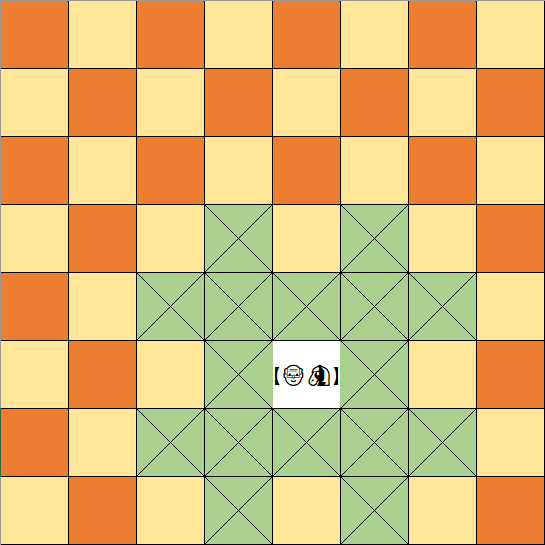
\includegraphics[width=1.5in]{inprob.png}
\end{figure}
\paragraph{}绿色区间不可以放其它的$hippocentaur$。可以证明,对于任意$2n\times 2n$的棋盘,最多放$n\times n$个$hippocentaur$(证明?你还想要证明?)
\paragraph{}定义$f(n)$表示$2n\times 2n$的棋盘放$n\times n$个$hippocentaur$的方案数,给定$n$求$f(n)$,答案对998244353取模。
\paragraph{输入格式}
\paragraph{}从\emph{hippocentaur.in}中读入数据
\begin{itemize}
\item 一行一个整数$n$
\end{itemize}
\paragraph{输出格式}
\paragraph{}输出到\emph{hippocentaur.out}中
\begin{itemize}
	\item 一行一个整数表示$f(n)$
\end{itemize}
\paragraph{样例输入}
\begin{lstlisting}
2
\end{lstlisting}
\paragraph{样例输出}
\begin{lstlisting}
25
\end{lstlisting}
\paragraph{子任务}
\paragraph{}对于$100\%$的数据,满足$n\le 2\times 10^7$
\begin{center}
	\begin{tabular}{|c|c|c|c|}
		\hline
		Subtask编号&分值&性质\\
		\hline
		1&15&$n\le 3$\\
		\hline
		2&10&$n\le 50$\\
		\hline
		3&15&$n\le 1000$\\
		\hline
		4&60&\\
		\hline
	\end{tabular}	
\end{center}

\clearpage
\begin{center}
	\large{Count}
\end{center}
\paragraph{题目描述}
\paragraph{}给定$n,k$,定义一个图是美丽的,当且仅当一号点度数$\leq k$。
\paragraph{}求出$n$个点有标号的任意美丽连通图个数(没有重边自环),对$998244353$取模。
\paragraph{输入格式}
\paragraph{}从\emph{count.in}中读入数据
\begin{itemize}
\item 一行两个整数$n,k$
\end{itemize}
\paragraph{输出格式}
\paragraph{}输出到\emph{count.out}中
\begin{itemize}
	\item 一行一个整数表示答案
\end{itemize}
\paragraph{样例输入}
\begin{lstlisting}
4 2
\end{lstlisting}
\paragraph{样例输出}
\begin{lstlisting}
30
\end{lstlisting}
\paragraph{子任务}
\paragraph{}对于$100\%$的数据,满足$n\le 500,k\le 75$
\begin{center}
	\begin{tabular}{|c|c|c|c|}
		\hline
		Subtask编号&分值&性质\\
		\hline
		1&10&$n,k\le 6$\\
		\hline
		2&10&$n,k\le 40$\\
		\hline
		3&20&$n\le 100, k\le 10$\\
		\hline
		4&20&$n\le 200, k\le 50$\\
		\hline
		5&40&\\
		\hline
	\end{tabular}	
\end{center}
\end{document}